Un bloque de masa $m$ = 160 gramos, está en contacto con un resorte que se comprime $X$= 8.0 cm, como se observa en la figura de este problema. Partiendo del reposo en $A$, el bloque es empujado por el resorte, abandonándolo en $B$, y se dirige hacia la rampa, cuya altura máxima es $H$ = 50 cm.
\begin{enumerate}
    \item Sabiendo que la constante del resorte es $k$ = 200 N/m, determine la energía potencial elástica en $A$.
    \item Suponiendo que la fricción sea despreciable y usando la conservación de la energía, demuestre que el bloque no conseguirá subir hasta lo alto de la rampa.
    \item Determine la altura $b$ que el bloque puede alcanzar al subir la rampa (considere $g$ = 10 m/s$^2$).
\end{enumerate}
\begin{figure}[htb]
  \centering
  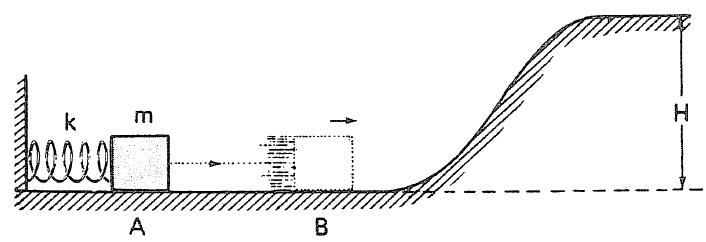
\includegraphics[scale=0.4]{figuras/fig_alvarenga_p389_13.png}
  \caption{Problema 7}
\end{figure}
